% \documentclass[%
%  reprint,
%  amsmath,amssymb,
%  aps,
% ]{revtex4-2}
\documentclass[%
 reprint,
 amsmath,amssymb
 aps,
]{revtex4-2}

\usepackage{float}

\usepackage{graphicx}% Include figure files
\usepackage{dcolumn}% Align table columns on decimal point
\usepackage{bm}% bold math
\usepackage{physics}
\setlength{\parskip}{\baselineskip}%
\usepackage{siunitx}
\usepackage[inline]{asymptote}
\usepackage{multirow}
\usepackage{tikz}
\usepackage{pgfplots, pgfplotstable}
% \def\bibsection{\section*{\refname}} 
\usepackage{hyperref}
\usepackage{natbib}
\bibliographystyle{unsrtnat}

\pgfplotsset{compat=1.3}
\begin{document}

% \preprint{APS}

\title{Verifying Amplitude Dependance of the Period of a Homemade Pendulum}% Force line breaks with \\

\author{QiLin Xue}

\date{\today}% It is always \today, today,
             %  but any date may be explicitly specified

\begin{abstract}
This experiment analyzed the effects of large amplitudes on the period of a home-made pendulum. The data for the period was obtained by releasing the pendulum at an angle near $90^\circ$ and measuring how the period changes as the pendulum decays. Both a quadratic and quartic fit was applied. Both agreed with theory, with the quartic fit giving coefficients of $\beta=0.064\pm 0.007$ and $\zeta=0.0029 \pm 0.0008$ for the coefficients of the second order and fourth order amplitude correction terms. The motion was extremely symmetric, and provides a good reference point for future experiments where mass and length dependance will be tested.
\end{abstract}

%\keywords{Suggested keywords}%Use showkeys class option if keyword
                              %display desired
\maketitle

%\tableofcontents
\section{Introduction and Modifications}
The previous experiment was able to calculate the $Q$ factor of a homemade pendulum, which measures how slowly the amplitude decays over time. That experiment is only valid for small angles, as it made the assumption that the period stays constant. In reality, the period is dependant on the amplitude $\theta_0$ via the relationship:\cite{doi:10.1119/1.1457310} %CITE
\begin{equation}
    T = 2\pi\sqrt{\frac{\ell}{g}}\left(1+\frac{1}{16}\theta_0^2+\frac{11}{3072}\theta_0^4+\cdots\right)
    \label{eq:correct-model}
\end{equation}
where $\ell$ is the distance from the center of mass of the pendulum to the pivot. Using a similar experimental setup as last time, I will analyze how well this model describes the behaviour of the pendulum. Several suggestions were made from the previous report, and the following were able to be implemented:
\begin{itemize}
    \item The pendulum is attached to the pivot using two strings, one on each side of the pendulum, to prevent the rope from twisting which may create unwanted coupling effects.
    \item The GoPro video setting was increased to 100 FPS, in order to decrease blur allowing AutoTracker to accurately track the motion of the pendulum.
\end{itemize} 
To account for environmental constraints preventing the pendulum to go to $90^\circ$, the rope length was decreased from $163.5 \pm 0.1\si{\centi\meter}$ to $107.5 \pm 0.1\si{\centi\meter}$. Using $7\pm 1\si{\centi\meter}$ (derived in the previous report) as an estimate of the center of mass of the pendulum with respect to the string, then the change in the distance to the center of mass is around:
\begin{equation}
    f\equiv \frac{\ell_\text{cm,new}}{\ell_\text{cm,before}}=\frac{115\pm 1\si{\centi\meter}}{165\pm 1\si{\centi\meter}} \approx 0.70 \pm 0.01
    \label{eq:}
\end{equation}
where the uncertainty is obtained adding in quadrature. The $Q$ factor is proportional to $Q \propto \sqrt{\ell}$, so the new $Q$ factor should be around:
\begin{equation}
    Q_\text{new} = Q_\text{before}\sqrt{f} = 259 \pm 8
    \label{eq:}
\end{equation}
One suggestion that was not implemented was the recommendation of using a more dense object than a filled water bottle, to reduce effects from air resistance. This suggestion was ultimately rejected for a practical reason: I wish to examine the effects of mass on the motion of the pendulum later on, and I wish to do so without affecting the cross sectional area of the pendulum. Variable scientific weights cannot accomplish that.
\section{Method}
The setup of the pendulum was exactly the same as the previous experiment, except the initial angle was near $90^\circ$, and was left to swing until it was nearly stopped. The camera was set very far away in order to capture the entire motion of the pendulum. Because of this, no optical corrections were found to be necessary.

As the amplitude decreases, it is predicted that the period would decrease as well. To reduce time uncertainties and statistical fluctuations, half-period measurements were made by measuring the time over a small intervals of amplitudes each with a range of $\Delta \theta = 0.2$. By finding the average of these half-amplitude measurements, I can get an estimate for the period at the midpoint (e.g. the average amplitude in each interval).

Even though this increases the uncertainty in the amplitude, the motivation is that for any small variation in the amplitude, the period can be approximated as linear with respect to amplitude such that a higher period from a higher amplitude would balance out the lower period from a lower amplitude, to arrive at a fairly accurate and precise average. In other words, if we sum up all period measurements that fall inside the interval $[\theta,\theta+0.2]$, the average period gives the period at the midpoint. As with last time, all calculations along with error propagation was done in a Python notebook, attached in Appendix B.
\section{Results}
\subsection{Q Factor}
The $Q$ factor was remeasured to be $Q=247 \pm 2$, following the same steps as before which loosely agrees with the theoretical predicted value of $Q=259\pm 8$. This is expected, since I have not drastically changed the setup. However, the air resistance was mostly linear in this experiment, as the natural logarithm of the angle gives a very nice linear fit when plotted with the time elapsed, as seen in figure \ref{fig:amplitude-vs-time}.
\begin{figure}[!h]
    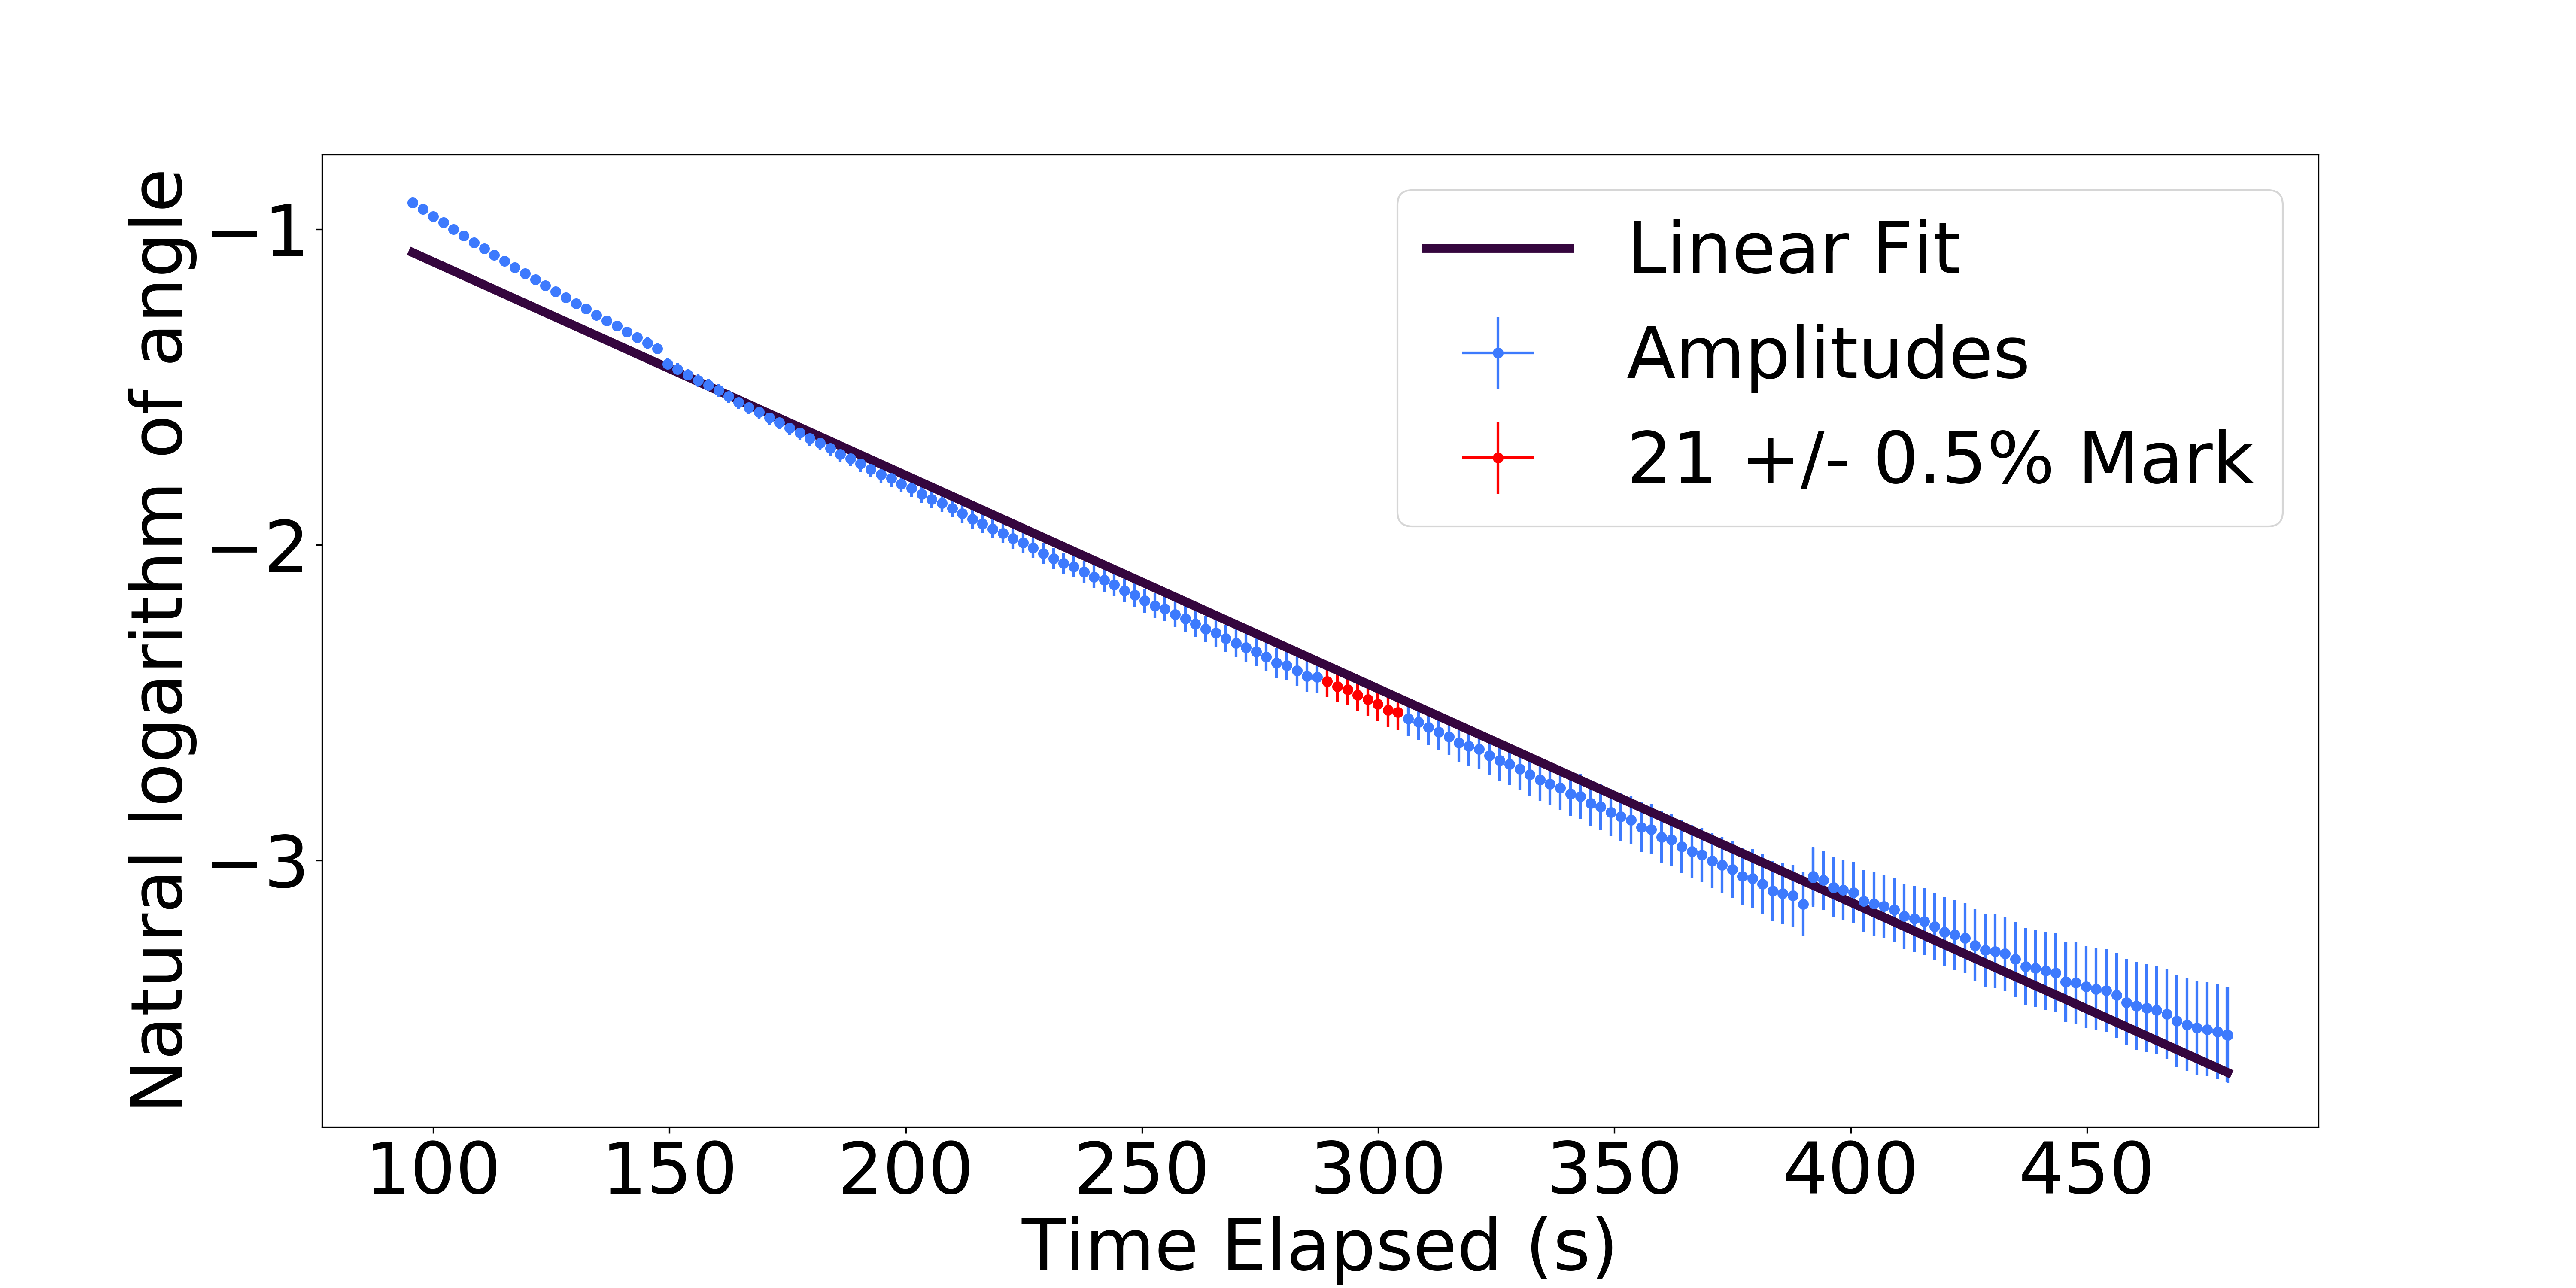
\includegraphics[width=\linewidth]{Figures/amplitude-vs-time-fitted.png}

    \caption{A plot of the natural log of the amplitudes with the line of best fit (where weights are set to the inverse of the standard deviation). The desired linear pattern was not seen. The quality of the fit is given by $R^2=0.99$. The red dots denote the amplitudes which fall within $21 \pm 0.5\%$ of the initial amplitude.}
    \label{fig:amplitude-vs-time}
\end{figure} 
I measured this value using the same steps as the previous experiment. Since my initial angle had a magnitude of $\theta_0=1.42 \pm 0.03$, which is considered a fairly large angle, I needed to ensure I was measuring the same value as last experiment. Thus, only the data after the pendulum has reached an amplitude of around $\theta_0\approx 0.357 \pm 0.007$ was used.

\subsection{Period}
In general, the data agrees very well with the model. Using the quadratic fit shown in figure \ref{fig:period-vs-amplitude}, my data suggests a relationship of:
\begin{equation}
    T = T_0\left(1+\alpha \theta_0 +\beta\theta_0^2\right)
    \label{eq:}
\end{equation}
with:
\begin{align}
    T_0 &= 2.140 \pm 0.005 \si{\second} \\ 
    \alpha &= -0.001 \pm 0.002\\
    \beta &= 0.0670 \pm 0.0007
\end{align}
which is reasonably close to the predicted values of:
\begin{align}
    T_0 &= 2.151 \pm 0.009 \si{\second} \\ 
    \alpha &= 0 \\ 
    \beta &= 0.0625
    \label{eq:}
\end{align}
Since the uncertainty of $\alpha$ is larger than the nominal value, we claim that the setup is mostly symmetric and that fluctuations in $\alpha$ could be easily caused by statistical uncertainties.
\begin{figure}[!h]
    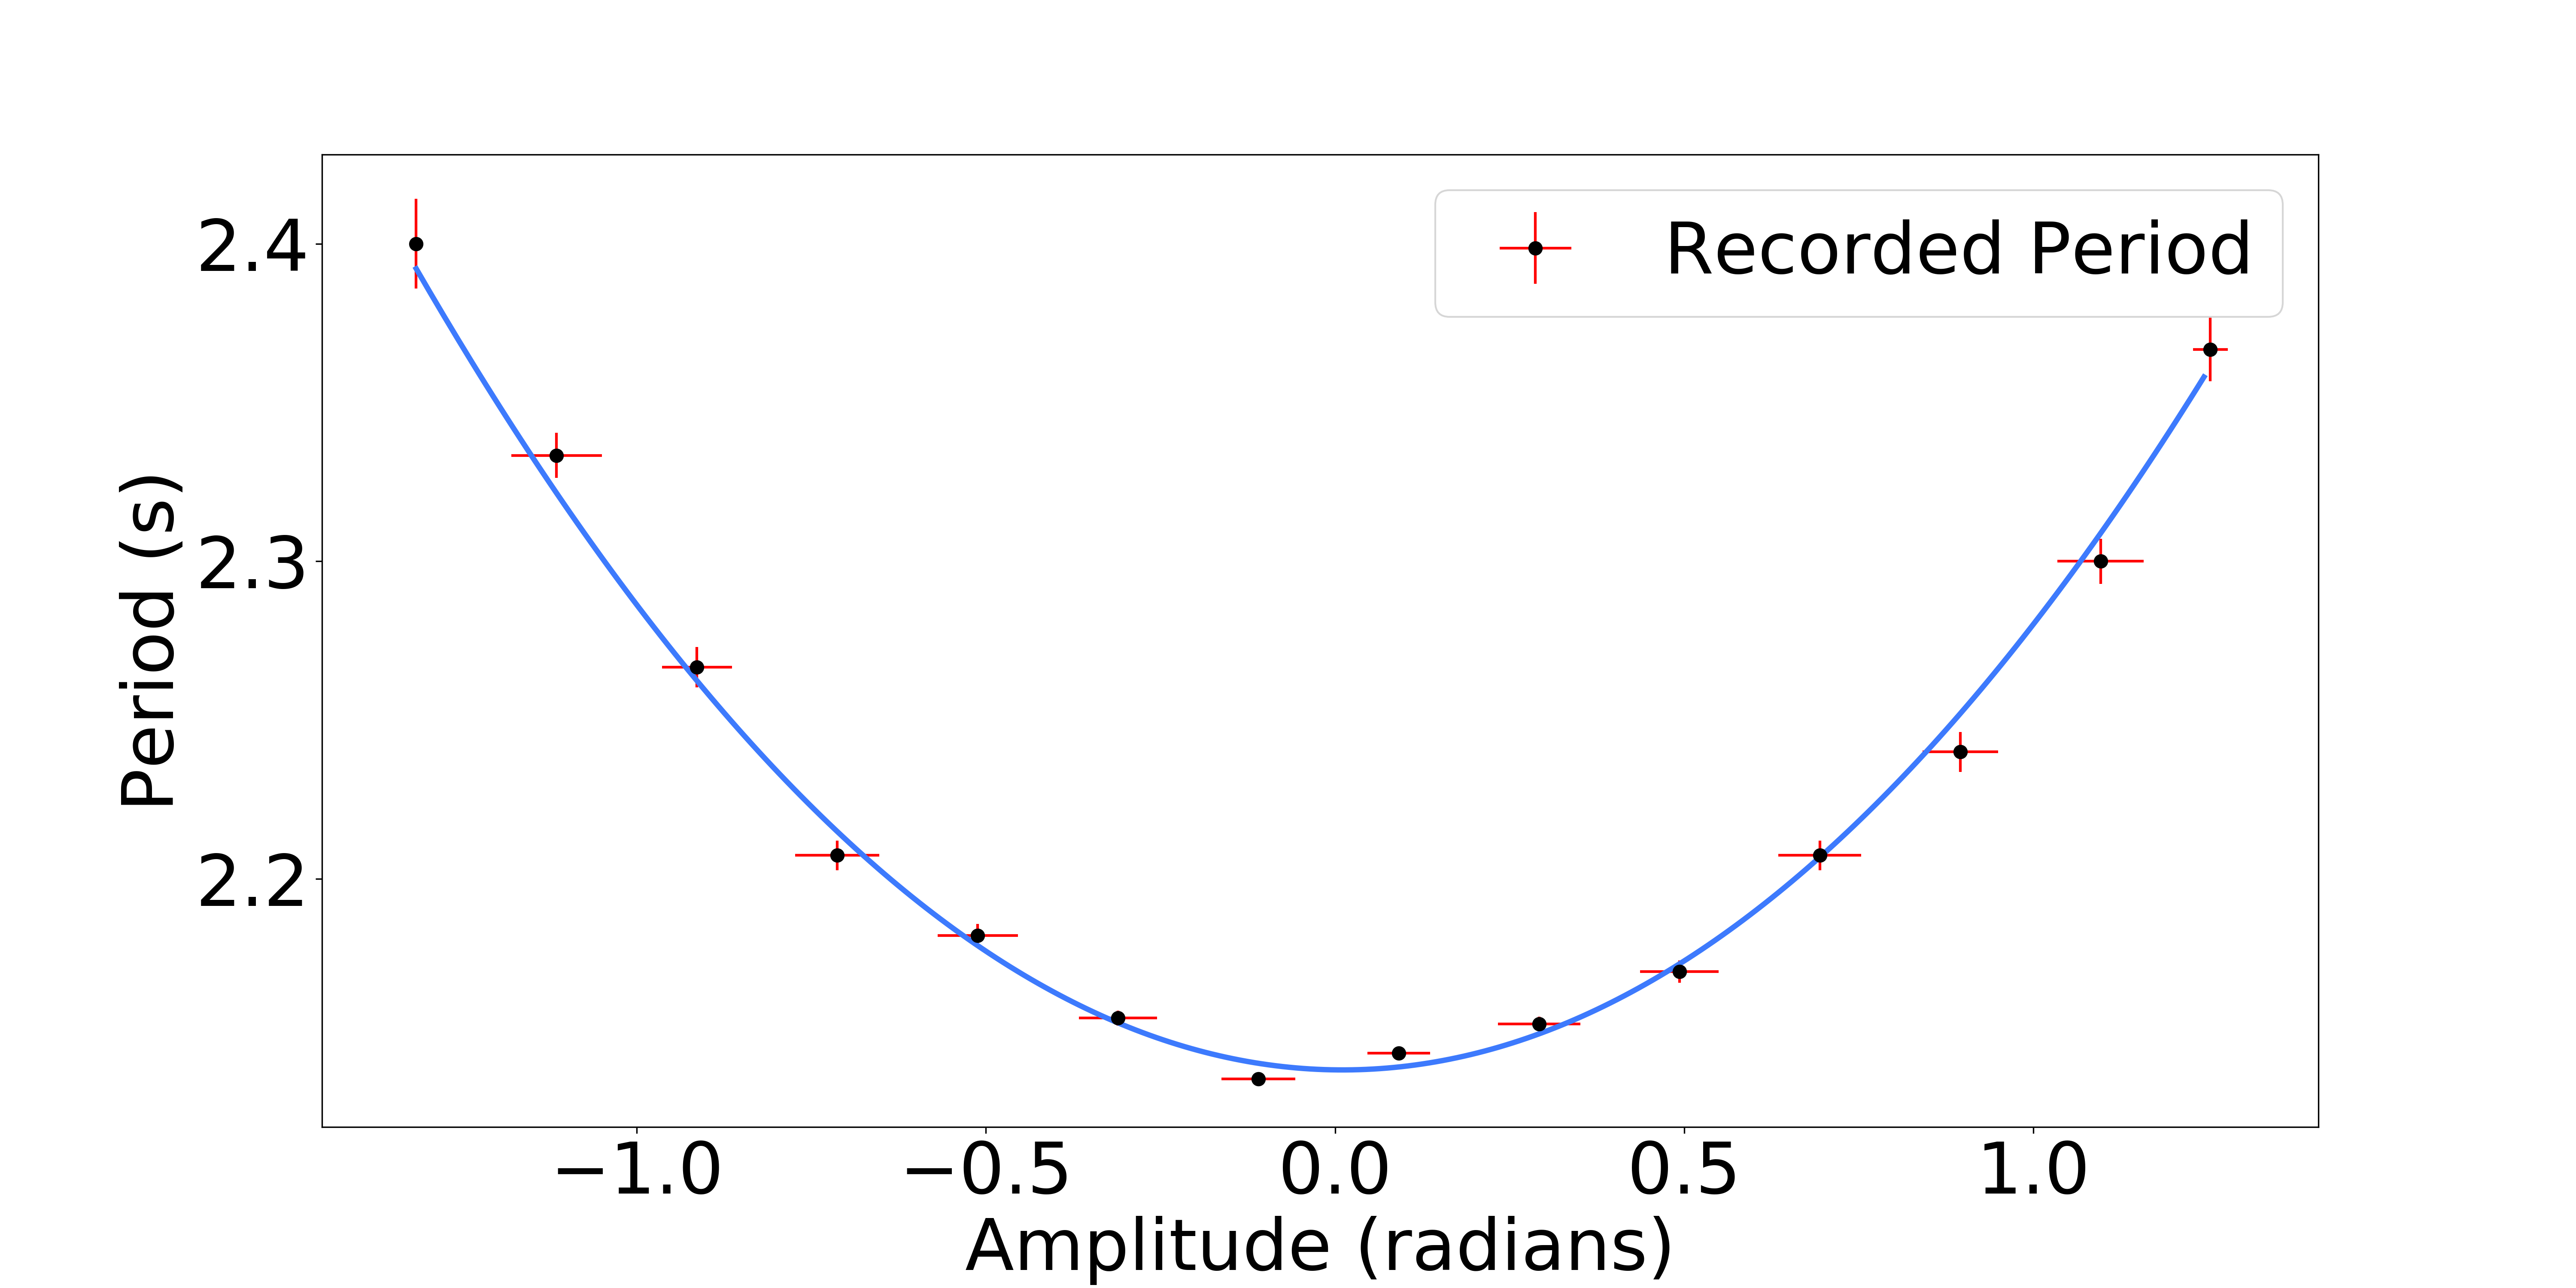
\includegraphics[width=\linewidth]{Figures/period-vs-amplitude.png}

    \caption{A plot of the period as a function of the amplitude. Note that the amplitude ranges from negative (to the left of the pivot) and positive (to the right), in order to test for asymmetry.}
    \label{fig:period-vs-amplitude}
\end{figure}
As a result, we can perform a linear regression by plotting the period against the square of the amplitude, as shown in figure \ref{fig:period-vs-amplitude-linear}. Using this linear regression, we verify that the period is $T_0=2.140 \pm 0.005$ and $\beta = 0.0670 \pm 0.0007$, as shown by considering a full quadratic fit. This confirms that the pendulum is exhibiting a very symmetric motion.
\begin{figure}[!h]
    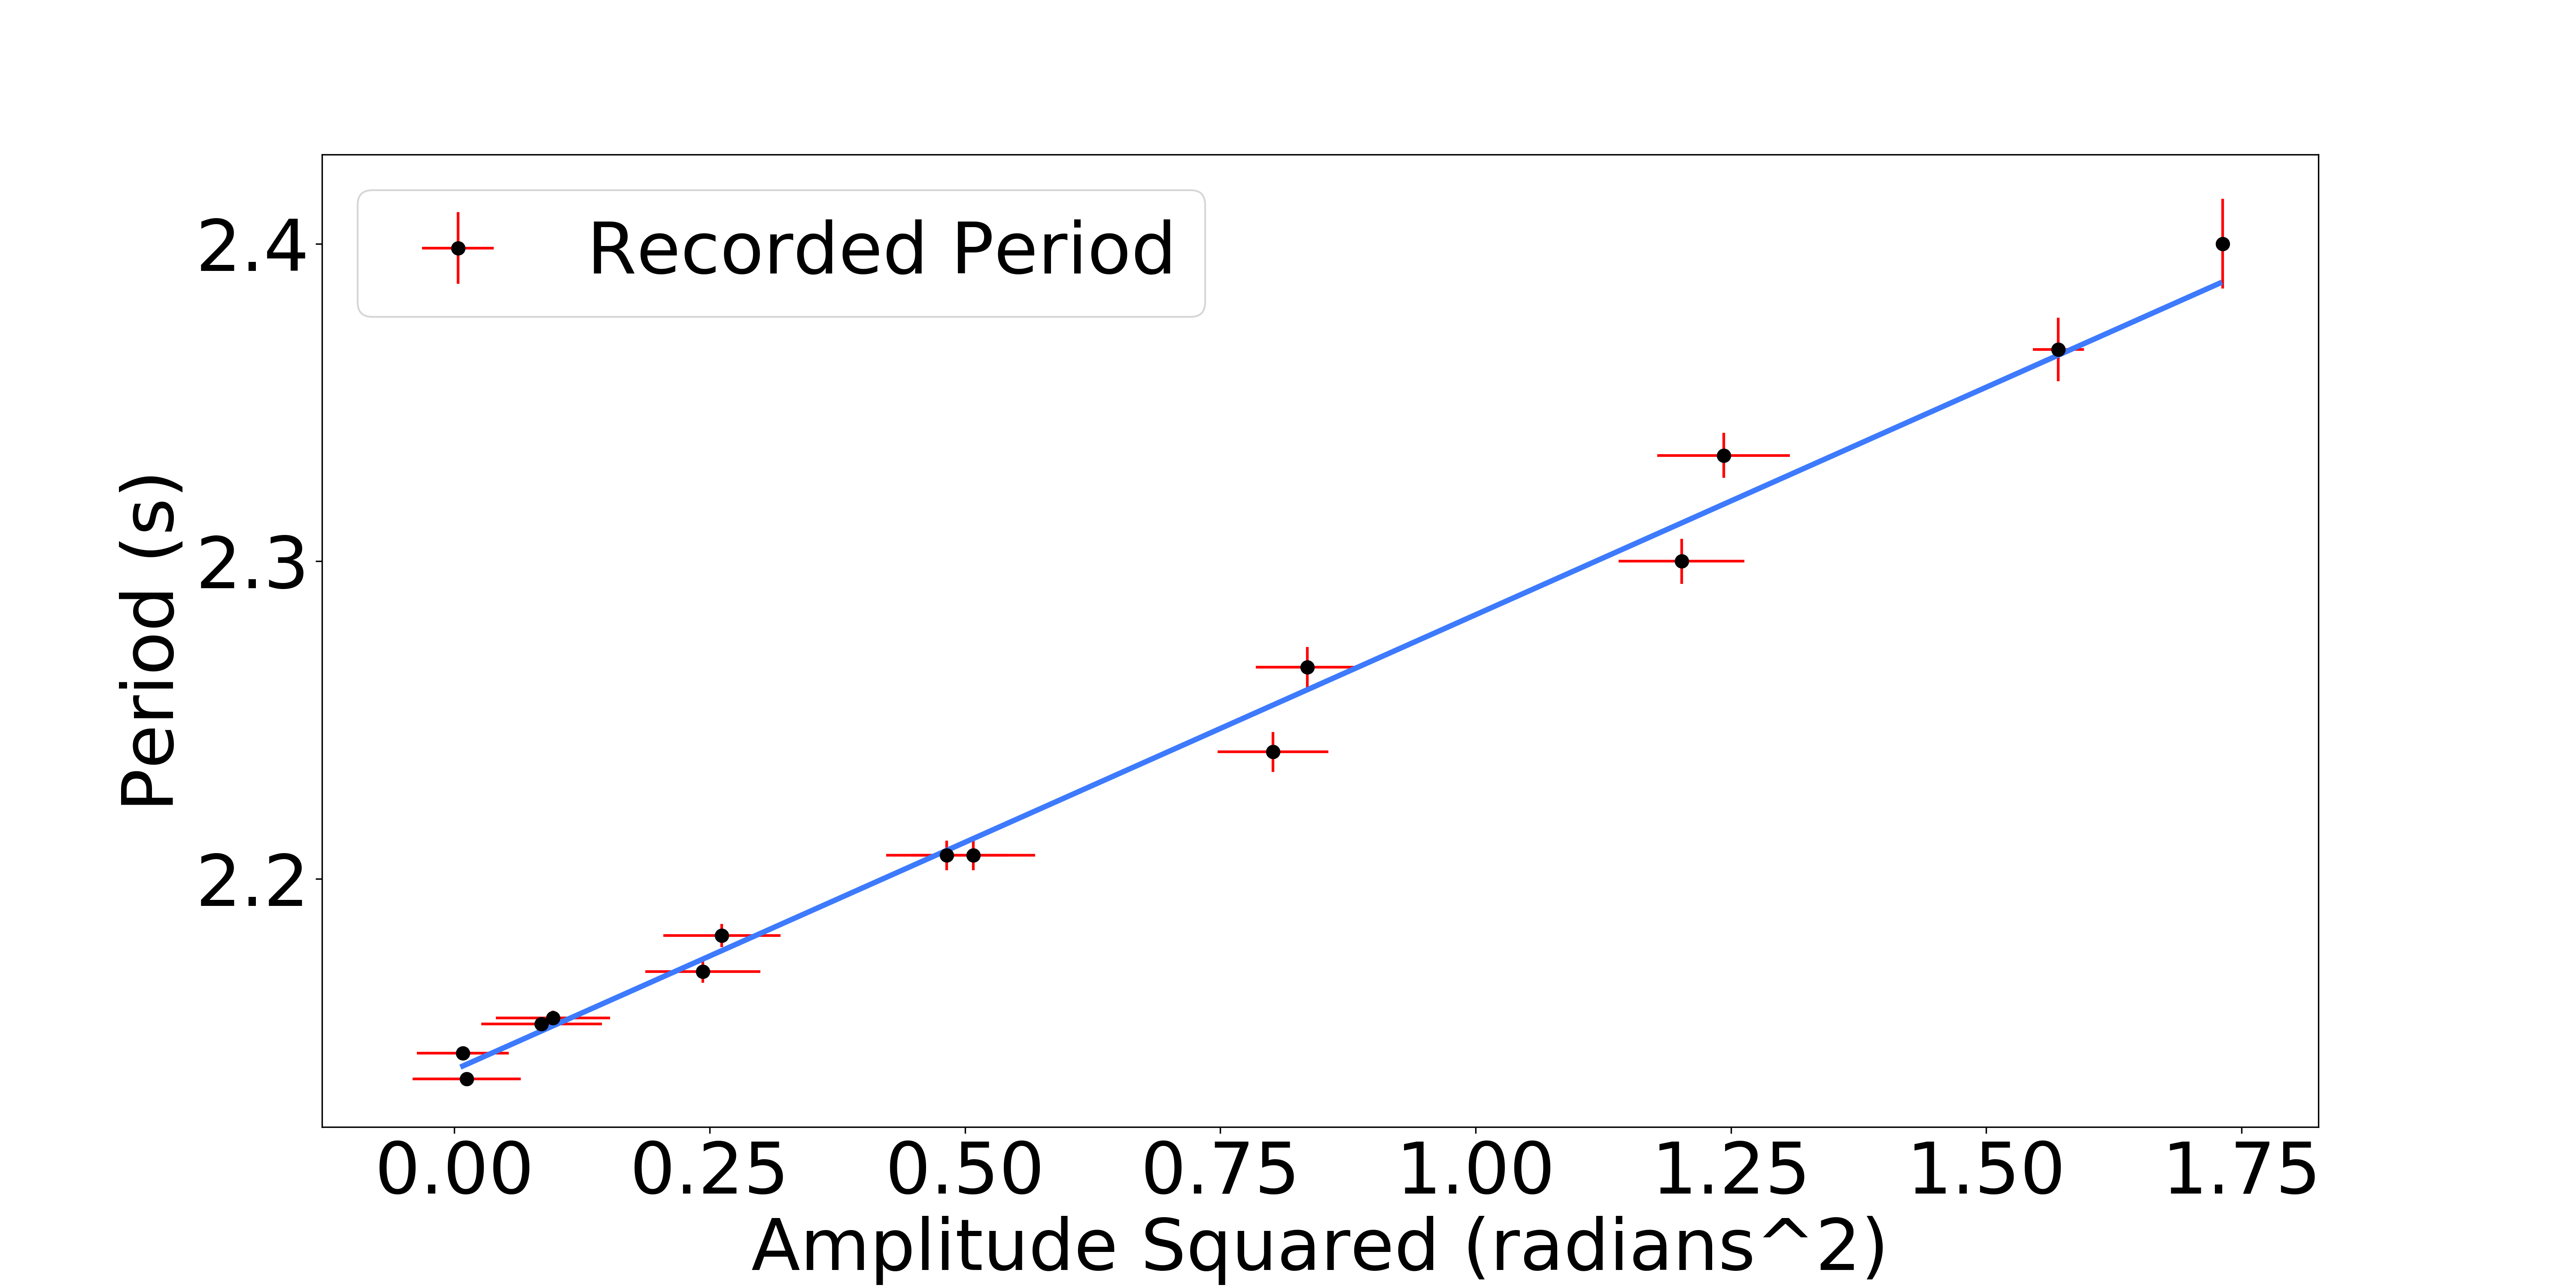
\includegraphics[width=\linewidth]{Figures/period-vs-amplitude-linear.png}

    \caption{A plot of the period as a function of the square of the amplitude. Similar value for $T_0$ and $\beta$ was obtained. The quality of the fit is given by $R^2=0.99$.}
    \label{fig:period-vs-amplitude-linear}
\end{figure}
\section{Discussion}
\subsection{Uncertainty of Amplitude Intervals}
Demanding that the amplitude intervals have a range of $\Delta \theta = 0.2$ is quite accurate, even for large angles. If we assume the model is valid, then I am essentially finding the average period from $\theta_1$ to $\theta_1+\Delta \theta$, or:
\begin{equation}
    T_\text{avg} = \frac{1}{\Delta \theta}\int_{\theta_1}^{\theta_1+\Delta \theta} T_0\left(1+\frac{1}{16}\theta^2\right)\dd{\theta}
    \label{eq:}
\end{equation}
via experimental sampling. For the measured value of $T_0$ and using $\theta_1=-\frac{\pi}{2}$, I get that the average period should be around $T_\text{avg}=2.430 \pm 0.007\si{\second}$. I then let this average be equal to the linear approximation, which on the other hand would yield the period at the midpoint:
\begin{equation}
    T_\text{avg,approx} = T_0\left(1+\frac{1}{16}\left(\theta_1+\frac{\Delta \theta}{2}\right)^2\right)
    \label{eq:}
\end{equation}
giving $T_\text{avg,approx}=2.390 \pm 0.007 \si{\second}$. Here, the relative error reaches a maximum of $1.6\%$ at $\pi/2$. This is reasonable since the relative error using a quadratic approximation versus a quartic approximation gives a relative error of $1.9\%$, which has the same size.

\subsection{Impact of Q Factor}
Qualitatively, the $Q$ factor describes how slowly the system decays, so the higher the $Q$ factor, the more data points there are in each interval, which decreases the time uncertainty of each measurement.

A Q factor of $247\pm 2$ is sufficiently high such that for angles less than $70^\circ$, each interval has at least four data points, and for even smaller angles such as $35^\circ$, there were at least eight 10 data points.

Unfortunately, the decay at the very start was extremely rapid and only one measurement was able to be made for the initial angle. However, due to the high frame rate used, the uncertainty was still only $1\%$. It might be tempting to try to apply the $Q$ factor to the start of the motion, but it is only valid for small angles. At large angles, the effective $Q$ factor becomes smaller, and can drop by a factor of four.
\subsection{Uncertainties}
Overall, this experiment was conducted extremely well, with physical parameters such as the period agreeing with the predicted value. With the changes mentioned in the Introduction, several uncertainties were reduced:
\begin{itemize}
    \item Coupling Effects: There is no more rotation, so this effect has been eliminated completely.
    \item \textit{Tracker}: By nearly doubling the frame rate, and having a bottle that does not rotate, \textit{Tracker} had less error identifying where the pendulum was. I estimate this error to be one third the dimensions of the cap, which corresponds (as calculated in Python) to an average angular uncertainty of $0.3^\circ$ degrees.
\end{itemize}
The length uncertainty remains the same and is now the biggest source of uncertainty when determining the physical parameters such as the period. In the next lab, I would like to measure the center of mass of the bottle to a greater degree of accuracy, which will especially be important as water is removed or added from inside since that could affect the location of the center of mass. I will need to quantify for the change in the location of the center of mass as the mass of the pendulum is varied.

Finally, there are tiny fluctuations in the period as a function of amplitude. While part of the reason is due to an inaccurate model (see the below section), there were certain flaws in the experimental setup. Due to human error, I could not align and orient the bottle perfectly in line with its trajectory, causing some rotation at the start. Although there were two strings that quickly ensured the rotation stopped, the motion was still a bit chaotic at the start. In future labs, I should start the pendulum above my intended initial angle to let the chaotic effects settle down and create accurate markings to ensure I am releasing the pendulum from the right spot. 
\subsection{Small Angle Approximation Validity}
In this section, we will check if the quadratic approximation
\begin{equation}
    T = 2\pi\sqrt{\frac{\ell}{g}}\left(1+\frac{1}{16}\theta_0^2\right)
    \label{eq:}
\end{equation}
is valid, and at which angles the simple harmonic oscillator (SHO) formula can be used:
\begin{equation}
    T = 2\pi\sqrt{\frac{\ell}{g}}
    \label{eq:}
\end{equation}
We can achieve this by attempting a quartic fit, as shown in figure \ref{fig:period-vs-amplitude-quartic}. A quartic fit gives the fit of:
\begin{equation}
    T = T_0\left(1+\alpha\theta_0+\beta\theta_0^2+\gamma \theta_0^3+\zeta \theta_0^4\right)
    \label{eq:}
\end{equation}
and parameters:
\begin{align}
    T_0 &= 2.14 \pm 0.01 \\ 
    \alpha &= 0.002 \pm 0.004 \\ 
    \beta &= 0.064 \pm 0.007 \\ 
    \gamma &= -0.006 \pm 0.003 \\ 
    \zeta &= 0.0029 \pm 0.0008
    \label{eq:}
\end{align}
As predicted, the coefficients of the odd powers $\alpha$ and $\gamma$ are close to zero, with their uncertainties being approximately the same as their nominal values. Meanwhile, the value of $\beta$ has improved to $0.064\pm 0.007$, which has a relative error of less than $3\%$! This is an improvement from the $7\%$ relative error when $\beta=0.0670 \pm 0.0007$ was used. Additionally, the value of $\zeta$ has a relative error of $19\%$ with respect to the theoretical value of $\zeta_\text{theory}=\frac{11}{3072}\approx 0.0036$.
\begin{figure}[!h]
    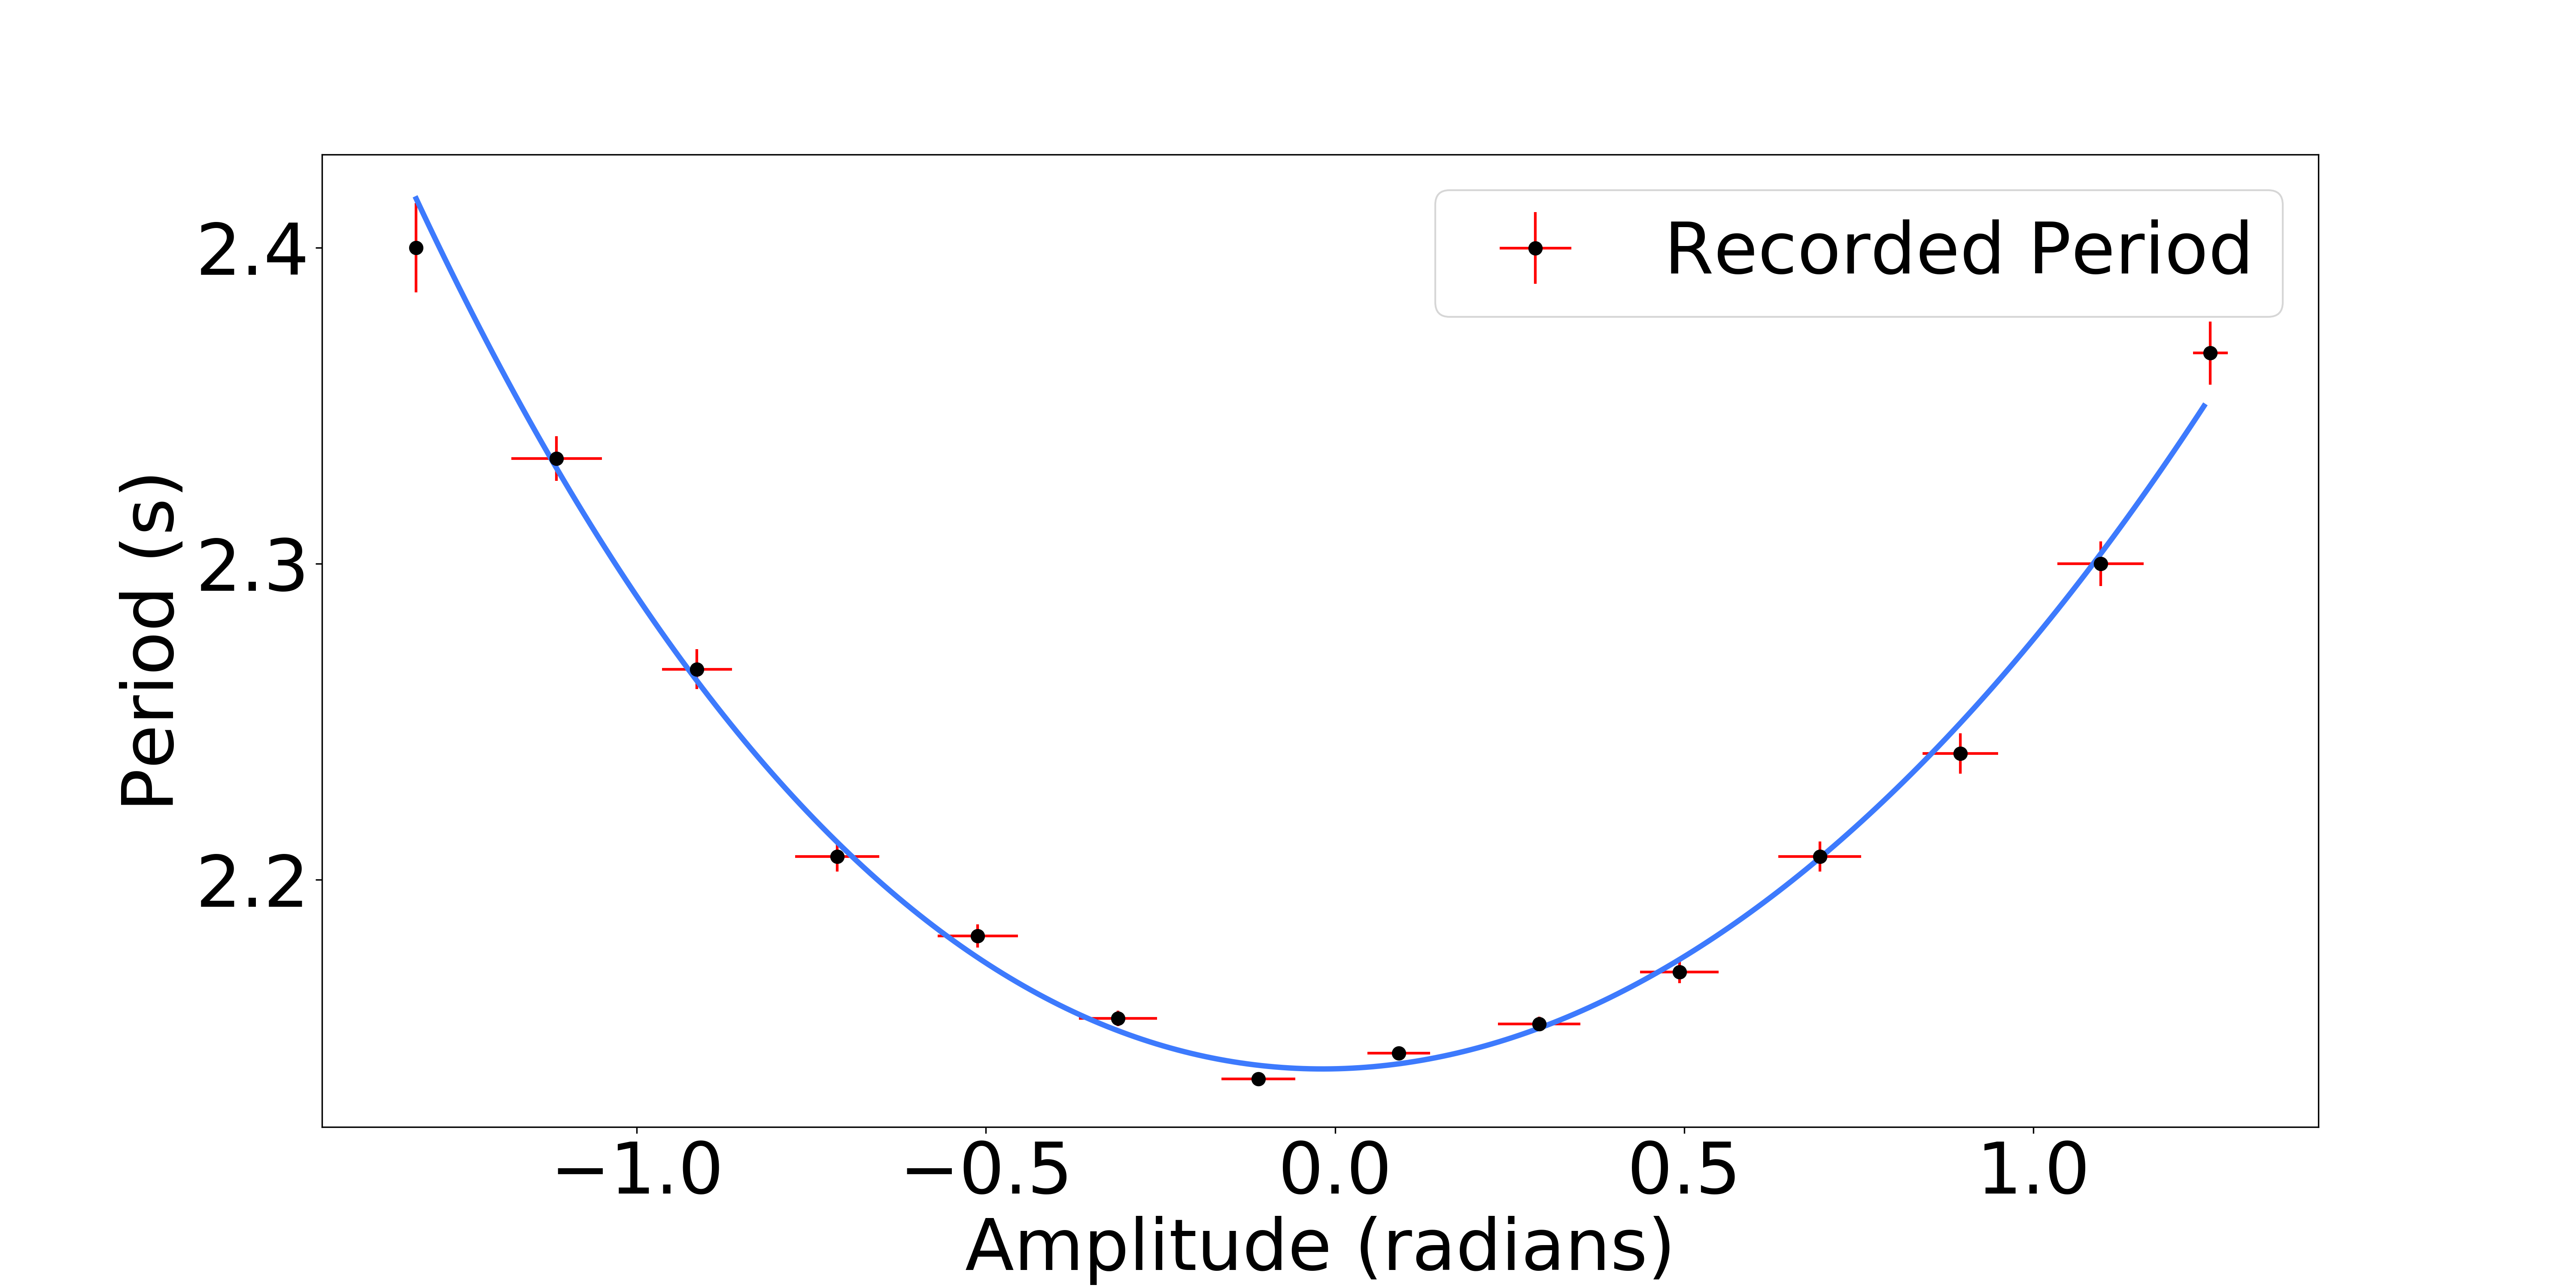
\includegraphics[width=\linewidth]{Figures/period-vs-amplitude-quartic.png}

    \caption{A plot of the period as a function of the amplitude, when fitted to a quartic function.}
    \label{fig:period-vs-amplitude-quartic}
\end{figure}
While this may seem like a large error, the theoretical value is actually within the statistical margins for $\zeta$. The likely values for $\zeta$ take on from $\zeta \in [0.0021,0.0037]$, and $\zeta_\text{theory}$ is contained in this range. I predict that if more accurate data was collected, especially at higher angles, then the nominal value of $\zeta$ will get closer to the predicted value and the uncertainties would decrease.

Since the coefficients become closer to their predicted value, this further supports that the model presented in equation \ref{eq:correct-model} is valid, which we can use to determine when we can use a quadratic model instead of a quartic model. We can do this by demanding the relative error in the period to be less than the time uncertainty divided by the period $\frac{\Delta t}{T} = 0.0023\si{\second}$, or:
\begin{equation}
    \frac{\frac{11}{3072}\theta^{4}}{1+\frac{1}{16}\theta^{2}+\frac{11}{3072}\theta^{4}} \le 0.0023
    \label{eq:}
\end{equation}
which gives the maximum angle to be $\theta_\text{max,quadratic}=0.911$ or $52.2^\circ$. Meanwhile, the maximum angle in which we can use the SHO formula instead of the quadratic approximation is given by when their relative error is under the time uncertainty as well:
\begin{equation}
    \frac{\frac{1}{16}\theta^{2}}{1+\frac{1}{16}\theta^{2}} \le 0.0023
    \label{eq:}
\end{equation}
which corresponds to an angle of $\theta_\text{max,SHO}=0.194$ or $11.1^\circ$. The relative error was chosen to be $\Delta T/T$ in an attempt to be as objective as possible. These angles represent the maximum angle at which the current apparatus can no longer detect a difference between the two models. Depending on the degree of precision needed, we may be happy with a relative error of $1\%$, in which case the angles at which a quadratic and SHO approximation can apply are $\theta_\text{max,quadratic}=76.2$ and $\theta_\text{max,SHO}=28.0^\circ$, respectively.
\section{Conclusion}
The purpose of the lab was to verify if the homemade pendulum built in the previous experiment follows the model presented in equation \ref{eq:correct-model}. The model turned out to be extremely accurate, and the parameters determined from the quartic fit agrees with the theoretical values.

A few changes were made between this experiment and the previous one to remove external effects and allow measurements to be made more precisely. However, there are still a few flaws in the experimental design. In future experiments, I would like to accurately measure the center of mass of the bottle, and develop a system to minimize the initial perturbations.

\bibliography{citations}

\onecolumngrid
\appendix
\section{Python Script and Data}
For script was written in Python through a Jupyter notebook, which is available to be viewed \href{https://github.com/QiLinXue/pendulum-labs/blob/main/lab2/Data%20Analysis.ipynb}{here}. It consists brief descriptions of the code, as well as descriptions of how optical corrections were done. Automatic error propagation is included.

For practical reasons, I cannot include the $140,000$ data points in this report, but they are made available \href{https://github.com/QiLinXue/pendulum-labs/blob/main/lab2/data.txt}{here}. It consists of three columns: time, $x$-position, and $y$-position. The origin is set to the equilibrium position of the pendulum.
\end{document}